\section{Experiments}

\subsection{Experiment Environment}
We implement our model using Python 3.6, Tensorflow 1.12 and Keras 2.2.
The model is trained on a single NVIDIA TITAN X (Pascal) GPU in each experiment on Ubuntu 16.04 OS.


\subsection{Dataset}
We use the public dataset CelebA\upcite{celeba}, which contains 202,599 facial images and 40 labelled attributes for each face.
We align and crop the facial images into three-channel(RGB) images of 128×128 pixels and then divide them into training sets, test sets and verification sets according to the ratio of 8:1:1.
For the 40 attributes in the dataset, we select 7 of them: 'gender', 'skin color', 'hair color', 'beard', 'wear glasses', 'young', 'lipstick' attribute to verify the feasibility of the model.

\subsection{Experimental Items}
\begin{itemize}
\item In order to obtain a suitable model structure and training hyperparameters, we have designed multiple sets of comparative experiments to test the effects of different improvement projects.
\item In order to verify that our model can generate plausible facial images according to input conditions and it has practicability, we have set up experiments of generating and adjusting facial images.
\item To prove that our method is cheaper to use, we have also set up a set of model size comparison experiments.
\end{itemize}

\subsection{Training Details}

We use the Adam\upcite{adam} optimizer to optimize the network.
The learning rates of the discriminator, the generator and the adjustor network are set to $1\times10^{-4}$.
$\beta1$ and $\beta2$ select the default configuration in Adam's\upcite{adam} paper, which is respectively 0.5 and 0.9.
The $\alpha$ in Leaky ReLU\upcite{leaky} is set to $0.3$.
The dropout\upcite{dropout} rate is set to $0.5$.
The encoder network is fixed when training the adjustor network.
The $\lambda$ in both the generator and the adjustor network is set to 0.02.
We use 93-dimensional noise vector and 7-dimensional attributes vector as input.
Use 32 images training set for training.
A total of 20 training sessions are used.
In each batch, the generator is used to generate the image first.
Then the discriminator is used to identify the image and adjusted by the adjustor network.
The calculation results of discriminator are on gradient penalty.
The losses of the discriminator, the generator and the adjustor network are calculated respectively. 
Then the respective optimizers separately performs backpropagation and optimizes network weight parameters.
In the partition training, the overall model training and the partition training are performed in a 4:1 ratio.

\subsection{Evaluation Metric}
It is difficult to evaluate the performance of generative models (e.g., GANs).
In our experiments, we choose the recently proposed metric Fr\'echet Inception Distance\upcite{fid} (FID) to evaluate our experiments.
It considers not only the synthetic data distribution but also how it compares to the real data distribution.
It directly measures the distance between the synthetic data distribution $p(.)$ and the real data distribution $p_r(.)$.
In practice, images are encoded with visual features by the inception model.
Assuming the feature embeddings follow a multidimensional Gaussian distribution,
    the synthetic data's Gaussian with mean and covariance $(m, C)$ is obtained from $p(.)$ and the real data's Gaussian with mean and covariance $(m_r, C_r)$ is obtained from $p_r(.)$.
The difference between the synthetic and real Gaussians is measured by the Fr\'echet distance, \emph{i.e}., $FID = ||m-m_r||_{2}^{2} + Tr\left(C + C_r - 2(CC_r)^{1/2}\right)$. Lower FID values mean closer distances between synthetic and real data distributions.
To compute the FID score for a unconditional model, 30k samples are randomly generated. To compute the FID score for a text-to-image model, all sentences in the corresponding test set are utilized to generate samples. \upcite{stackgan}


\subsection{Experiment Result}
\subsubsection*{More Efficient Generation}


Table \ref{result_speed} shows that the image generation speed of LittleGAN and DCGAN\upcite{dcgan}.
It runs on the computer with an Intel Core i7-6700 CPU.
It shows that the generate speed of LittleGAN is much faster.
It also means that LittleGAN will get higher real-time performance when deployed on computer or mobile devices.

\begin{table}
    \caption{Generate Speed Comparison}
    \label{result_speed}
    \centering 
    
    \begin{threeparttable}
        \begin{tabular}{c|c}
            \hline
            Experiment Name & Time       \\ \hline
            DCGAN        &  11.50s$\pm$0.21s\\
            Final\tnote{*}        &  3.29s$\pm$0.20s\\
            16x-Filter\tnote{*}        & 2.02$\pm$0.14s \\
            Size-5x5\tnote{*}        &  4.85s$\pm$0.07s\\
            48x-Filter\tnote{*}        & 9.91s$\pm$0.25s  \\ \hline
        \end{tabular}

        \begin{tablenotes}
            \item The 200 facial image generation time usage of LittleGAN and DCGAN.
            \item[*] This means the experiment model is LittleGAN.
        \end{tablenotes}
    \end{threeparttable}
\end{table}
Table \ref{result_fid} shows the FID metric of each model.
Lower is better for the metric.
The result of LittleGAN is after training 20 epochs.
Each experiment of LittleGAN takes us about 13.5 hours.
The mode collapse occurs on the whole DCGAN\upcite{dcgan} after training 16 epochs,
    which leads to the failure of the network.
    So, we select the result of DCGAN\upcite{dcgan}after training 15 epochs.
It can be seen that with the improvements,
    LittleGAN gets a better score than DCGAN\upcite{dcgan}.
    It also shows that LittleGAN's performance of generation image is available.
We find some FID\upcite{fid} statistical data on CelebA\upcite{celeba} dataset from the paper "Are GANs Created Equal? A Large-Scale Study"\upcite{gan-compare},
    while their models output the image size of 64x64.
In that case, their metrics will be much bigger at the same condition of ours.

\begin{table}
    \centering
    \caption{FID Metric Comparison}
    \label{result_fid}
    \begin{threeparttable}
    \begin{tabular}{l|ccccc}
        \hline
        Exp. Name    & Kernel Size & Filter Num.   & Partition          & Norm.         & FID            \\ \hline
        Final*        & 3x3         & 24x           & $\surd$            & Instance      & 57.94$\pm$0.09 \\
        Batch*        & 3x3         & 24x           & $\surd$            & Batch         & 59.35$\pm$0.64 \\
        16x-Filter*   & 3x3         & 16x           & $\surd$            & Instance      & 62.82$\pm$0.40 \\
        48x-Filter*   & 3x3         & 48x           & $\surd$            & Instance      & 59.35$\pm$0.42 \\
        Size-5x5*     & 5x5         & 24x           & $\surd$            & Instance      & 56.99$\pm$0.24 \\
        No-Partition* & 3x3         & 24x           & $\times$           & Instance      & 64.22$\pm$0.46 \\ \hline
        DCGAN        & 5x5         & 64x           & $\times$           & Batch         & 77.57$\pm$1.27 \\ \hline
        VAE(64x64)   & -           & -             & $\times$           & -             & 85.7 $\pm$3.8**  \\
        BEGAN(64x64) & 3x3         & 128x          & $\times$           & -             & 38.9 $\pm$0.9**  \\
        WGAN-GP(64x64) & 5x5       & 128x          & $\times$           & Batch         & 30.0 $\pm$1.0**  \\ \lasthline
    \end{tabular}
    
    \footnote{}
    \begin{tablenotes}
        \item The FID metric comparison between serval models.
        \item[*] This means the experiment model is LittleGAN.
        \item[**] this means the FID result is calculated by the paper from Google Brain "Are GANs Created Equal? A Large-Scale Study" 
    \end{tablenotes}
\end{threeparttable}
\end{table}


\subsubsection*{More Stable}
Figure \ref{loss_part_on_d} and \ref{loss_dcgan_d} are the discriminator's loss changes of LittleGAN and DCGAN\upcite{dcgan}.
Figure \ref{loss_part_on_g} and \ref{loss_dcgan_g} are the generator's loss changes of LittleGAN and DCGAN\upcite{dcgan}.
To better measure the convergence speed of LittleGAN and DCGAN\upcite{dcgan},
    we use TensorBoard visualization tool to generate a loss map of the network during training.
By comparison, it can be found that compared with DCGAN\upcite{dcgan},
    the loss of our network changes more smoothly, the variance is smaller and is steadily decreasing.
While DCGAN\upcite{dcgan} often appears to have a fitting and lead to a sudden increase in loss.

\begin{figure}
    \begin{minipage}[t]{0.49\linewidth}
        \centering
        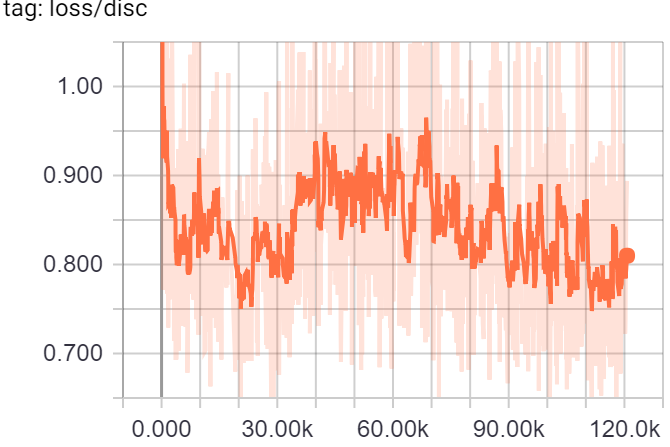
\includegraphics[width=\textwidth]{figures/loss_part_on_d.png}
        \caption{Loss line chart of LittleGAN's Discriminator (turn partition training on)}
        \label{loss_part_on_d}
    \end{minipage}
        \hfill
    \begin{minipage}[t]{0.49\linewidth}
        \centering
        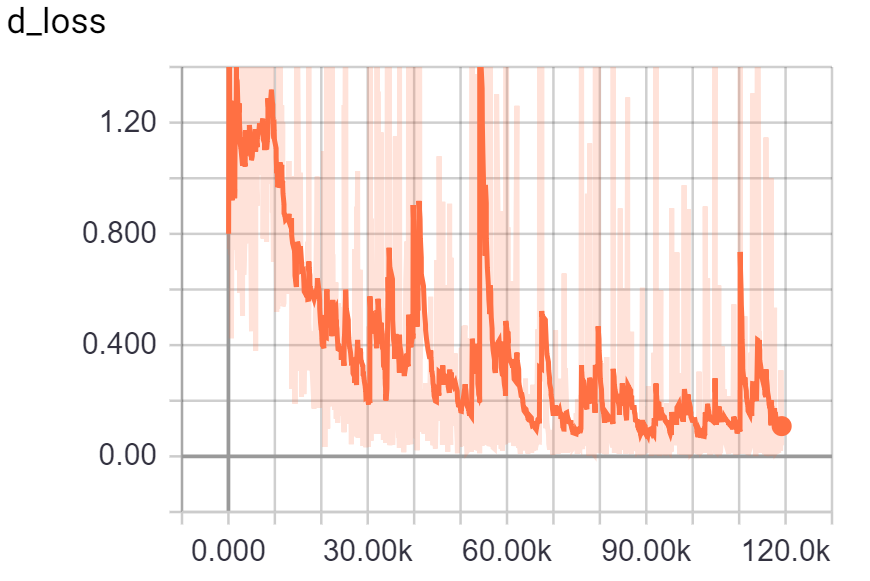
\includegraphics[width=\textwidth]{figures/loss_dcgan_d.png}
        \caption{Loss line chart of DCGAN's Discriminator}
        \label{loss_dcgan_d}
    \end{minipage}
\end{figure}

\begin{figure}
    \begin{minipage}[t]{0.49\linewidth}
        \centering
        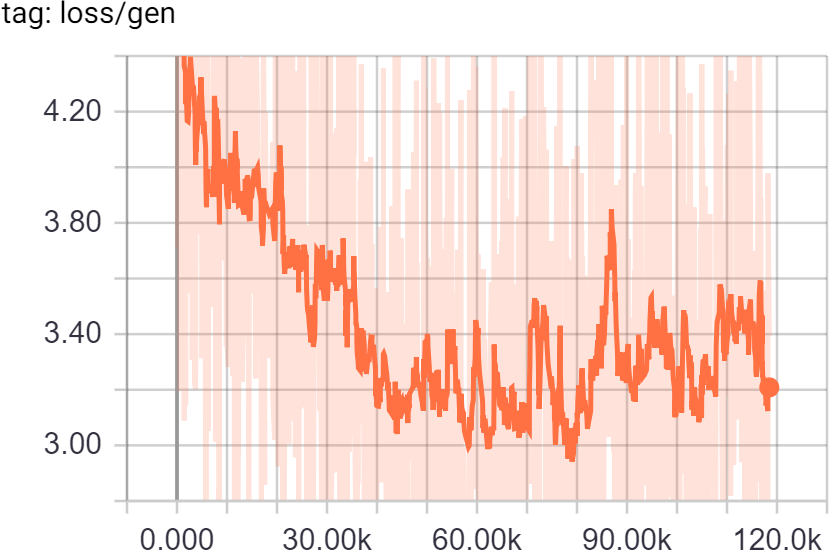
\includegraphics[width=\textwidth]{figures/loss_part_on_g.png}
        \caption{Loss line chart of LittleGAN's Generator (turn partition training on)}
        \label{loss_part_on_g}
    \end{minipage}
        \hfill
    \begin{minipage}[t]{0.49\linewidth}
        \centering
        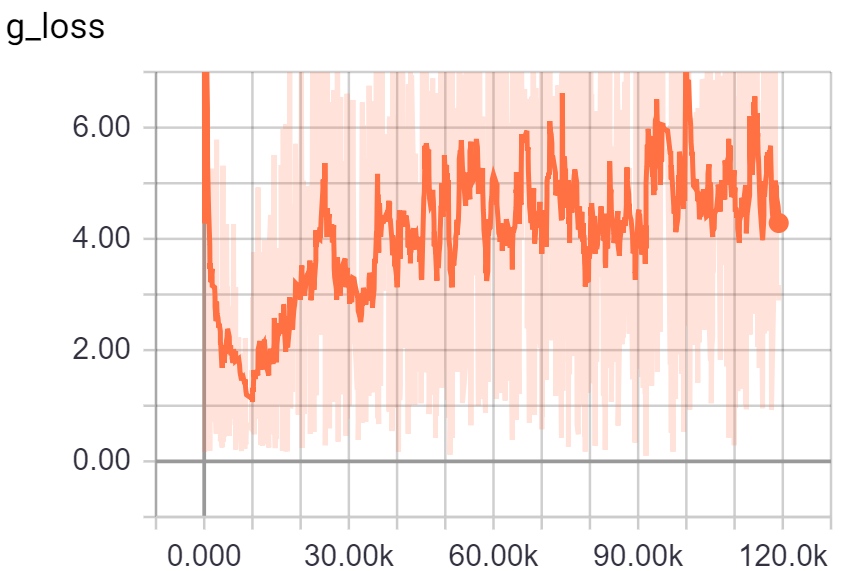
\includegraphics[width=\textwidth]{figures/loss_dcgan_g.png}
        \caption{Loss line chart of DCGAN's Generator}
        \label{loss_dcgan_g}
    \end{minipage}
\end{figure}

Figure \ref{littlegan_e15} and Figure \ref{dcgan_e15} are the test output of LittleGAN and DCGAN\upcite{dcgan} after training 15 epochs of training.
LittleGAN can output very authentic facial images after training 15 epochs.

\begin{figure}
    \begin{minipage}[t]{0.48\linewidth}
        \centering
        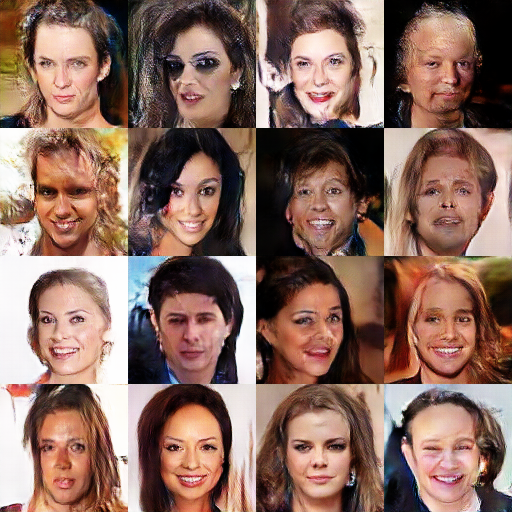
\includegraphics[width=\textwidth]{figures/result_littlegan_e15.png}
        \caption{Test result of LittleGAN after training 15 epochs}
        \label{littlegan_e15}
    \end{minipage}
        \hfill
    \begin{minipage}[t]{0.48\linewidth}
        \centering
        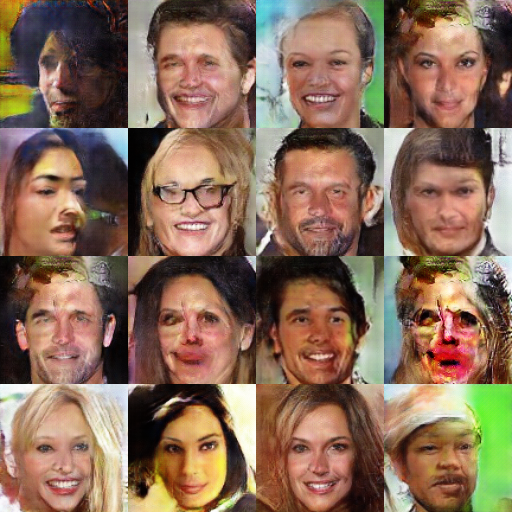
\includegraphics[width=\textwidth]{figures/result_dcgan_e15.png}
        \caption{Test result of DCGAN after training 15 epochs}
        \label{dcgan_e15}
    \end{minipage}
\end{figure}


\subsubsection*{Less Information Loss}
Figure \ref{adjust} is the test result of the generation and adjustment of the facial image.
It can be seen that when the image is roughly consistent, a single feature appears different from other images and other features are not lost.
Our network is able to adjust the specified features of the facial image.

\begin{figure}
    \begin{center}
    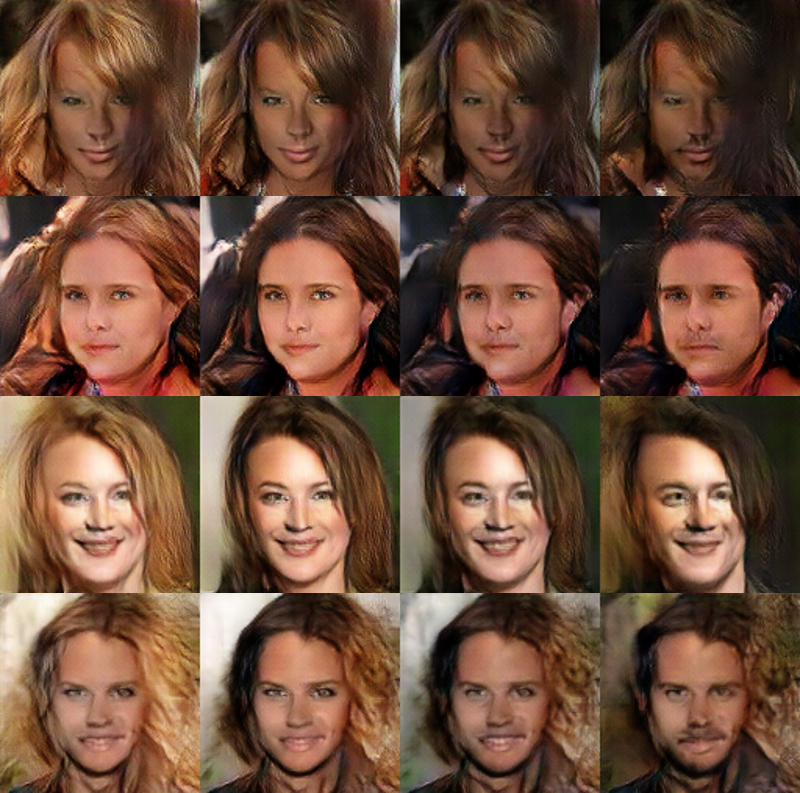
\includegraphics[width=0.49\textwidth]{figures/result_adjust_1.png}
    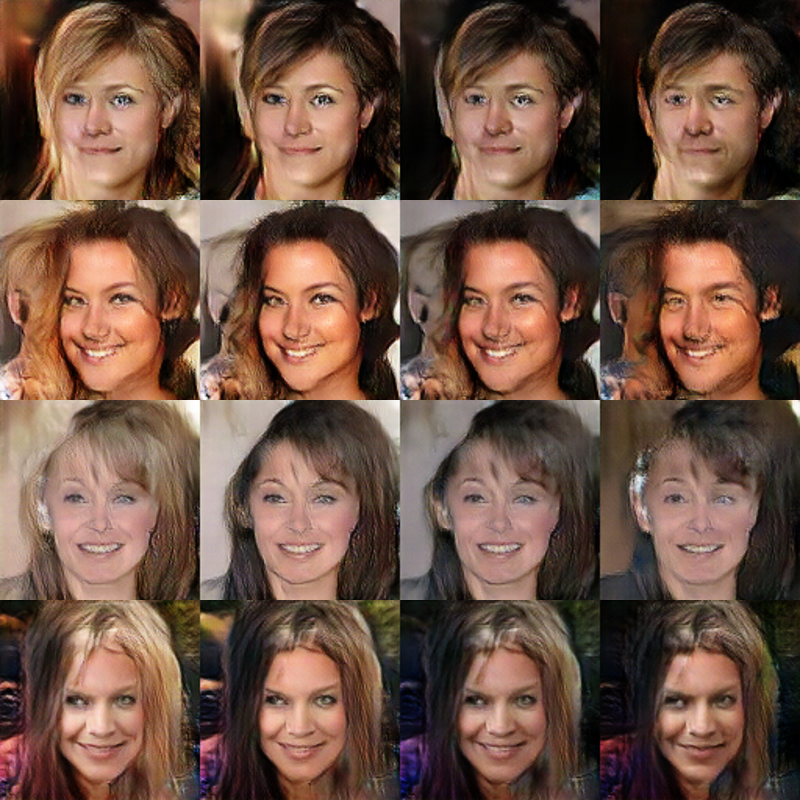
\includegraphics[width=0.49\textwidth]{figures/result_adjust_2.png}
    \caption{Adjustment test result of LittleGAN's Adjustor}
    \label{adjust}
    \end{center}
\end{figure}

\subsubsection*{Faster Convergence}
Figure \ref{littlegan_e1} and Figure \ref{dcgan_e1} show the results after training 1 epoch of training on LittleGAN and DCGAN\upcite{dcgan} on the CelebA\upcite{celeba} training set.
LittleGAN is able to produce clear and highly recognizable facial images after training 1 epoch of training.
Compared to DCGAN\upcite{dcgan}, we can see clearly that the images generated by LittleGAN are sharper and clearer.
It is also closer to the real image in color.
These means that the convergence of LittleGAN is faster than DCGAN at first.

\begin{figure}
    \begin{minipage}[t]{0.48\linewidth}
        \centering
        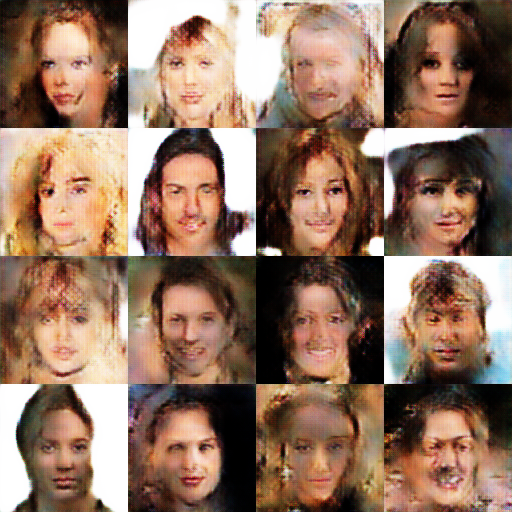
\includegraphics[width=\textwidth]{figures/result_littlegan_e1.png}
        \caption{Test result of LittleGAN after training 1 epoch}
        \label{littlegan_e1}
    \end{minipage}
        \hfill
    \begin{minipage}[t]{0.48\linewidth}
        \centering
        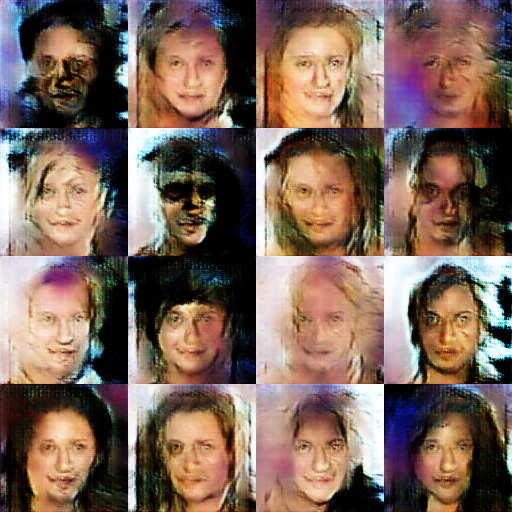
\includegraphics[width=\textwidth]{figures/result_dcgan_e1.png}
        \caption{Test result of DCGAN after training 1 epoch}
        \label{dcgan_e1}
    \end{minipage}
\end{figure}

Fig.\ref{loss_part_on_d}, Fig.\ref{loss_part_on_g}, and Fig.\ref{loss_part_on_u} show the changes of the loss of each components that turn partition training off, respectively.
Fig.\ref{loss_part_off_d}, Fig.\ref{loss_part_off_g}, and Fig.\ref{loss_part_off_u} show the changes of the loss of each components that turn partition training off, respectively.
It can be seen that the loss of the generator reaches the balance faster with partition training started.
 The loss of the discriminator also has a small amplitude and becomes stable.
Figure \ref{part_on} and Figure \ref{part_off} show the test output of the partition training on and off, respectively.
After training 20 epochs, with partition training on, image quality is improved under the same training amount.
These also means that the convergence of LittleGAN is faster than DCGAN at last.

\begin{figure}
    \begin{minipage}[t]{0.48\linewidth}
        \centering
        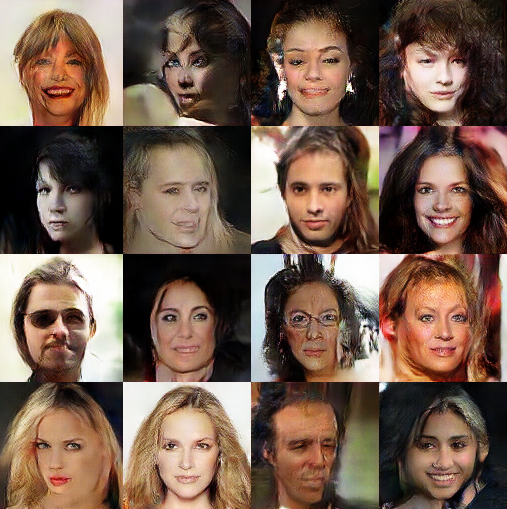
\includegraphics[width=\textwidth]{figures/result_part_on.png}
        \caption{Test result after training 20 epochs (turn partition training on)}
        \label{part_on}
    \end{minipage}
        \hfill
    \begin{minipage}[t]{0.48\linewidth}
        \centering
        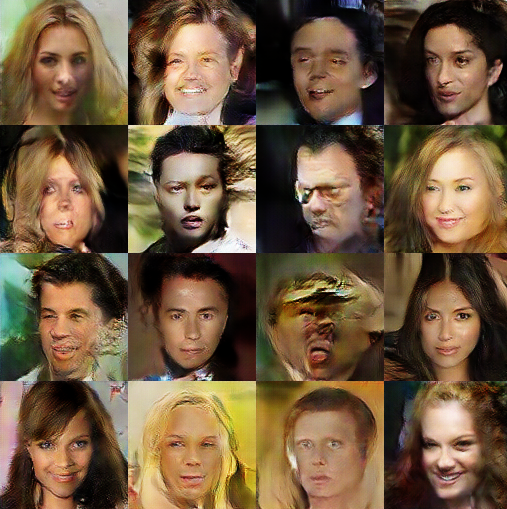
\includegraphics[width=\textwidth]{figures/result_part_off.png}
        \caption{Test result after training 20 epochs (turn partition training off)}
        \label{part_off}
    \end{minipage}
\end{figure}

\begin{figure}
    \begin{minipage}[t]{0.49\linewidth}
        \centering
        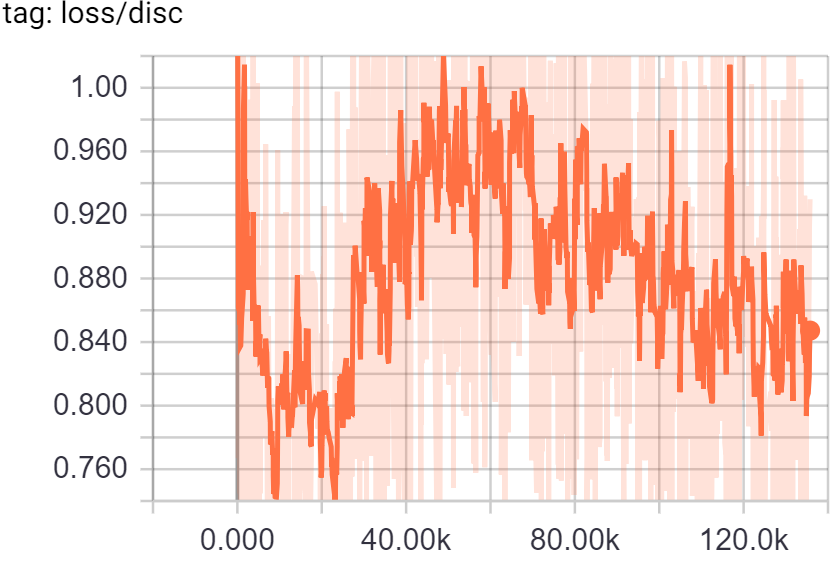
\includegraphics[width=\textwidth]{figures/loss_part_off_d.png}
        \caption{Loss line chart of LittleGAN's Discriminator (turn partition training off)}
        \label{loss_part_off_d}
    \end{minipage}
        \hfill
    \begin{minipage}[t]{0.49\linewidth}
        \centering
        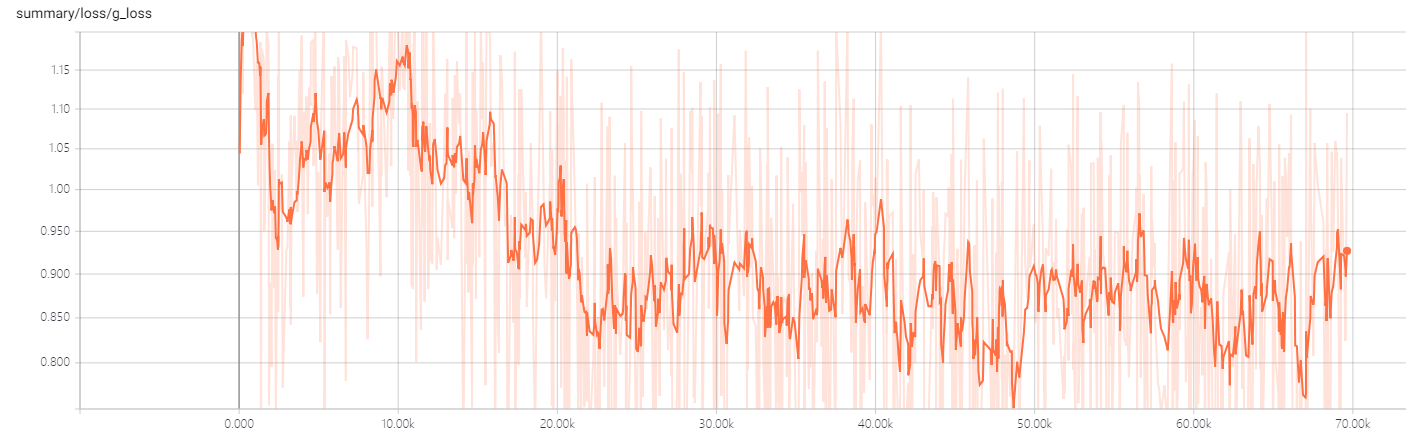
\includegraphics[width=\textwidth]{figures/loss_part_off_g.png}
        \caption{Loss line chart of LittleGAN's Generator (turn partition training off)}
        \label{loss_part_off_g}
    \end{minipage}
\end{figure}

\begin{figure}
    \begin{minipage}[t]{0.49\linewidth}
        \centering
        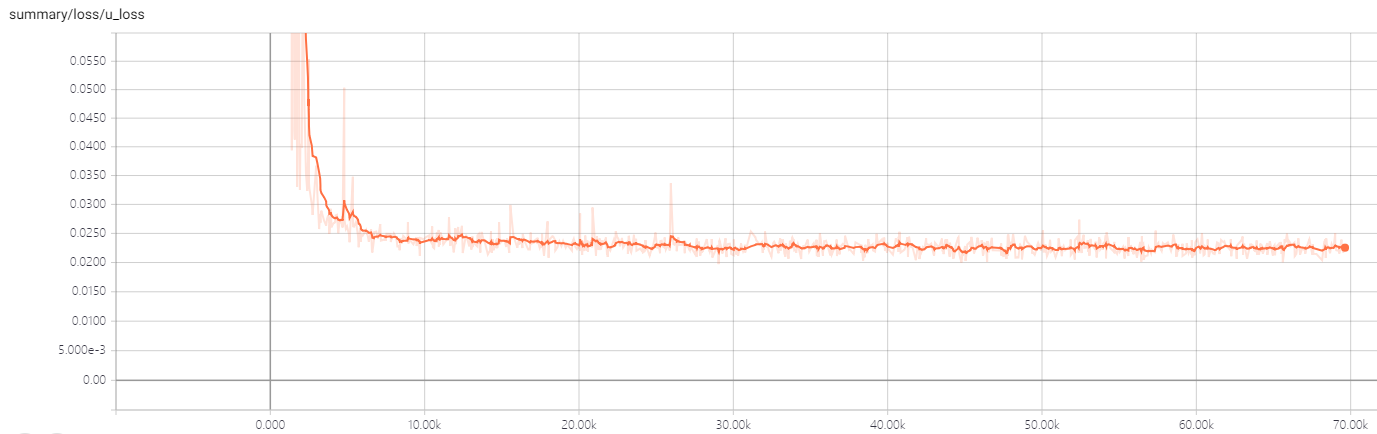
\includegraphics[width=\textwidth]{figures/loss_part_off_u.png}
        \caption{Loss line chart of LittleGAN's Adjustor (turn partition training off)}
        \label{loss_part_off_u}
    \end{minipage}
        \hfill
    \begin{minipage}[t]{0.49\linewidth}
        \centering
        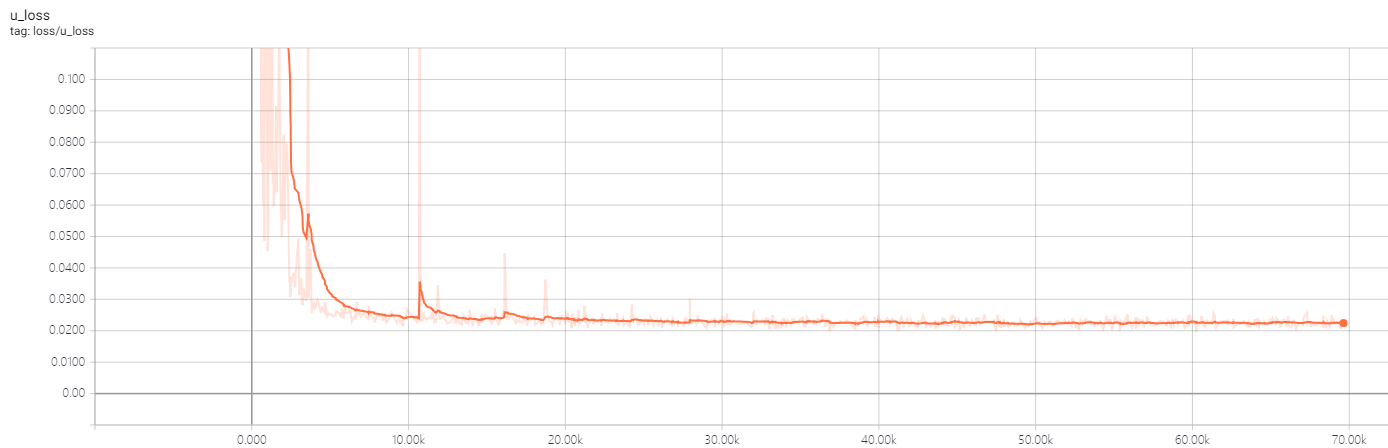
\includegraphics[width=\textwidth]{figures/loss_part_on_u.png}
        \caption{Loss line chart of LittleGAN's Adjustor (turn partition training on)}
        \label{loss_part_on_u}
    \end{minipage}
\end{figure}


\subsubsection*{Lower Use-cost}
We have used a variety of methods to reduce the size of model and the amount of computation.
We compare the model size of pix2pix\upcite{pix2pix}, DCGAN\upcite{dcgan} and LittleGAN when outputting the same size image (a three-channel color image of 128 × 128 pixels).
It is shown in Figure \ref{result_model_size}.
It can be seen that the size of LittleGAN is smaller and LittleGAN costs less.

\begin{figure}
    \begin{center}
    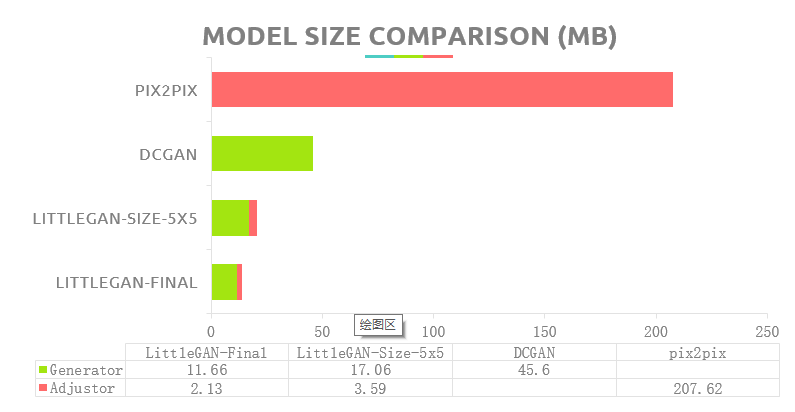
\includegraphics[width=\textwidth]{figures/result_model_size.png}
    \caption{Model Size Comparison}
    \label{result_model_size}
    \end{center}
\end{figure}



